
\chapter{System design}
\section{System overview} \label{sec:system}

\begin{figure}[h]
    \centering
    \vspace{-0.7cm}
    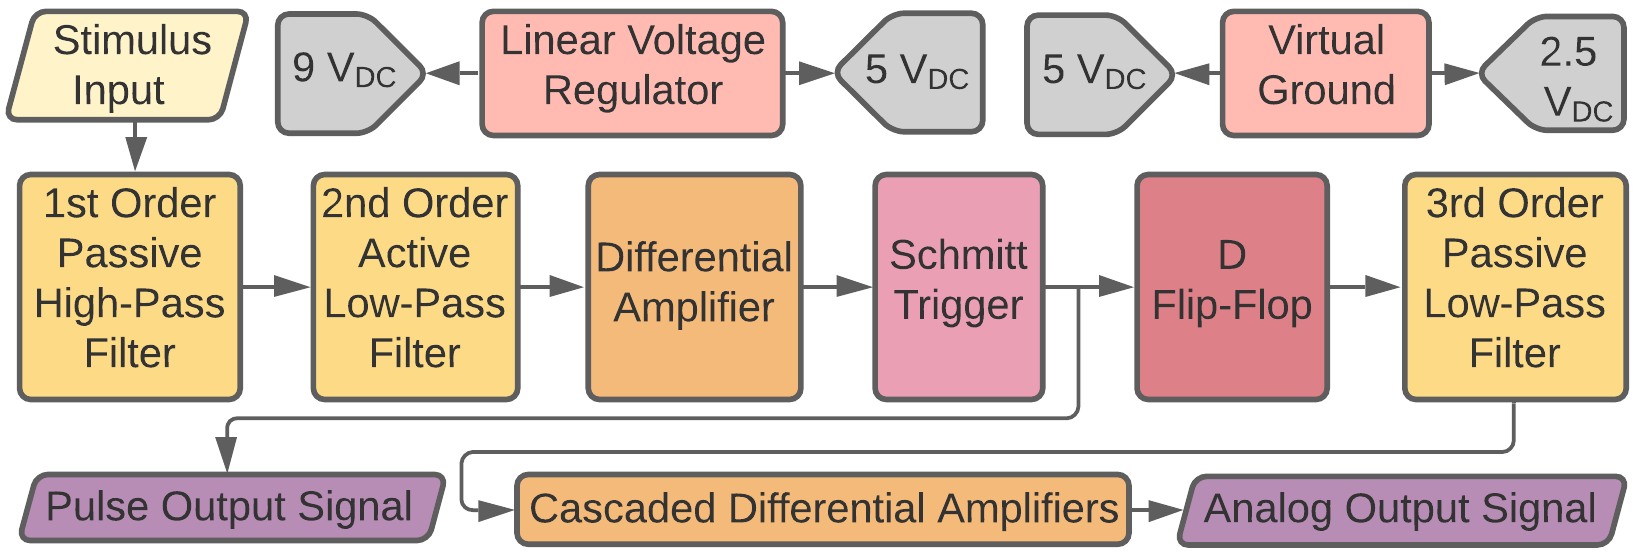
\includegraphics[width = 0.9\textwidth]{Figures/overview}
    \caption{System Diagram}
    \label{fig:overview}
\end{figure}

A heart-rate sensor is designed to receive an input signal from which pulses and analogue values are generated, corresponding to heart-beats and the heart-rate respectively. The aforementioned is achieved by voltage regulation, signal conditioning, pulse generation and conversion to analogue, as shown in figure \ref{fig:overview}. The circuit is powered by a voltage regulator \cite{prev} which can supply \SI{100}{mA}, of which \SI{12.8}{mA} is used for the temperature sensor - see E344 Assigment 1 \cite{prev} - leaving \SI{87.2}{mA} at \SI{5}{V}, mandating conservative current use. The input signal has an amplitude of insufficient magnitude for conversion, and is subject to noise, necessitating signal conditioning: a first order passive high-pass filter and a second order active low-pass filter attenuate both high- and low-frequencies. Chosen with maximal simplicity in mind to reduce cost and complexity, the filters still performing adequately. Thereafter, a differential amplifier produces a signal with a large amplitude and little noise. A Schmitt Trigger then outputs a pulse signal with a frequency corresponding to the heart-rate. The Schmitt Trigger was chosen as it provides a noise margin via hysteresis. An analogue voltage output is required for the microcontroller - filtering and peak detection using diodes was considered but discarded, as non-linear diodes result in extremely slow simulation. Rather, the pulse output signal was converted to a pulse-width modulated signal, where the frequency of the former determines the duty cycle of the latter. This was done as PWM signals lend themselves to conversion-to-analogue by simple filtering. The PWM signal was obtained by using a D Flip-Flop and a RC-circuit (see section \ref{sec:heartDesign}). A third order passive RC filter is then used - passive components reduce current usage and simulation time. The filter is of high order as to minimize noise, while meeting the settling time requirement. Finally, the signal was amplified to achieve the required range.